\documentclass[main.tex]{subfiles}
\begin{document}



\subsection{Verzovací systémy}
\label{git}
Verzovací systémy jsou nástroje pro uchovávání změn libovolných souborů v histori. Dále jsou používány k usnadnění vývoje nejčastěji softwarových projektů při týmovém vývoji. Je tedy možné kdykoli dohledat autora libovolné změny a stav souboru k danému datu. Verzovací systémy jsou nejčastěji používány pro zaznamenávání změn ve zdrojových souborech programů. Je však možné je použít k verzování libovolných dat.

Pro vývoj tohoto projektu byl využit verzovací systém git, který bude popsán níže.

Verzovací systémy lze dělit podle způsobu distribuce dat mezi vývojáři.

\subsubsection{Centralizované systémy}
Prní možností je centralizovaný systém, který pracuje s jedním hlavním servrovým úložištěm, k němuž uživatelé (vývojáři) přistupují a upravují jej. Většina operací s repozitářem vyžaduje připojení k onomu serveru.

\subsubsection{Distribuované systémy}
Oproti centralizovaným verzovacím systémům neexistuje centrální repozitář. Naproti tomu vlastní každý uživatel vlastní kopii projektu. Změny provedené uživatelem jsou poté sdíleny s ostatními typicky pomocí smluveného serveru. Tento server je však možné kdykoli zaměnit s libovolným jiným.

\subsubsection{Git}
Git je příkladem distribuovaného verzovacího systému. Je vyvíjen od roku 2005, kdy projekt započal Linus Torvalds, hlavní vývojář linoxového jádra, aby jej mohl udržovat. Předtím byl pro správu linuxového jádra používán verzovací systém BitKeeper, tehdy proprietární, dnes již open-source. \cite{web:wik:en:git} Git je používán pro správu malých projektů, včetně tohoto, tak i pro rozsáhlé projekty, jako například \href{https://github.com/blender/blender}{blender} nebo již zmíněné \href{https://github.com/torvalds/linux}{linuxové jádro}.

%Git je v informatice distribuovaný systém pro správy verzí. \cite{wik:git} Prakticky to znamená, že uchovává soubory v průběhu času a umožňuje kooperovaný vývoj projektů. Byl vytvořen Linusem Torvaldsem, hlavním vývojářem linuxového jádra, pro jeho správu. Nicémě dnes je používán v množství open source i proprietárních projektů. Před vznikem gitu byl používán proprietární verzovací systém BitKeeper. \cite{wik:git}


\subsubsection{Vlastnosti}
Následující požadavky byly klíčové při vývoji gitu a nadále se těmito vlastnostmi vyznačuje:
\begin{itemize}
\item Git významně podporuje paralelizaci vývoje v tzv. větvích (branch). Díky tomu lze pracovat na jednotlivých změnách např. v programu paralelně, aniž by došlo k promítnutí změny do hlavní verze programu. Až po otestování funkcionality může být přidána do hlavní větve programu (tzv. merge). 

\item Vyznačuje se vysokou efektivitou při práci se soubory, a proto je použitelný i u velkých projektů, aniž by operace trvaly nepřiměřeně dlouho.

\item Vysoká ochrana proti nechtěnému poškození souborů.

\end{itemize}
%Oproti jiným verzovacím systémům se vyznačuje decentralizovaností - téměř všechny operace s daty lzeprovádět, lokálně bez přístupu k internetu (až na operace pracující se vzdáleným servrem).
%Při vývoji gitu požadoval jeho autor, Linus Torvalds, následující vlastnosti:


		\begin{figure}[h]
			\centering
			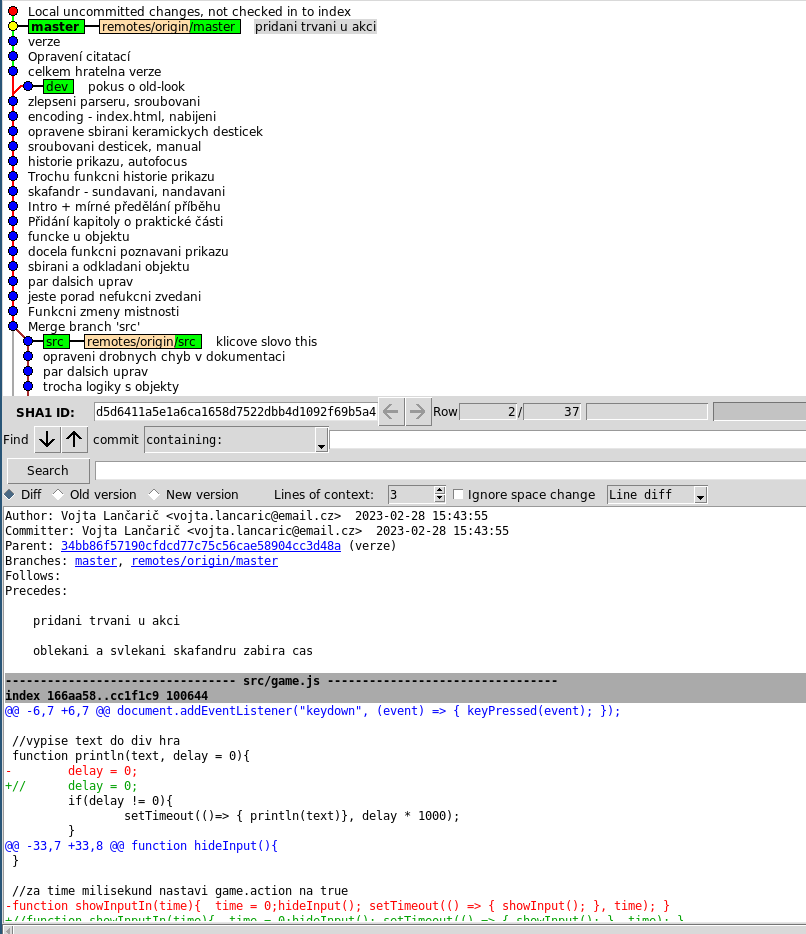
\includegraphics[width=.6\textwidth]{./git/git_history.png}
			\caption{Ukázka historie projektu v gitu}
		\end{figure}

%\subsubsection{fungování}

%\subsubsection{lokální operace}

\subsubsection{Použití v projektu}
Při vývoji tohoto projektu byl git použit jednak pro zaznamenávání provedených změn, užitečné zejména při samotném vývoji hry - psaní kódu, a také pro sdílení práce s vedoucím prostřednictvím webové stránky Github. Na \href{https://github.com/vojta006/mp}{této} webové adrese na nechází zdrojové kódy k práci.

\subsubsection{Github}
Github je webová služba umožňující sdílet a uchovávat gitové repozitáře (projekty), buďto jako soukromé (private), nebo veřejné (public). Uživatelům s opravněním umožňuje komentovat jednotlivé commity a klonovat repozitáře pro vlastní potřebu. 

\end{document}

